\section{Automação}
\label{sec:auto}

Automação consiste na execução automatica de um processo com o mínimo de
intervensão humana. Para a área de TI, a automação ocorre nos processos de
controle e administração de sistemas ou softwares~\cite{sharma:2015}.

Pode-se citar algumas das vantagens da automação~\cite{sharma:2015}:
\begin{itemize}
  \item Ajuda a reduzir a complexidade de um processo;
  \item Ajuda a reduzir possibilidade de erros humanos em tarefas
    repetitivas;
\end{itemize}

\citeonline{sharma:2015} aborda as necessidade de se adotar automação na área
de TI (Tecnologia da Informação) e relaciona com os conceitos como métodos
ágeis, entrega contínua, computação em nuvem, etc. Além disso, são citados
os benefícios da automação mapeados com as principais preocupações da industria
de TI. Algumas delas:
\begin{itemize}
  \item \textbf{Agilidade}: promove pontualizada de agilidade para a TI. Em conjunto
    com os métodos ágeis resulta em múltiplas implantações em um curto intervalo
    de tempo;
  \item \textbf{Escalabilidade}: a automação ajuda a transformar a infra-estrutura
    em códigos simples, ou seja, a construção, reconstrução e configuração é possível
    ser feita em poucos minutos;
  \item \textbf{Precisão de Implantação}: com a utilização de \textit{scritps}
    é possível realizar rápidas mudanças nas configurações de um ambiente
    obtendo os resultados esperados.
\end{itemize}

A automação, em conjunto com a cultura DevOps, consegue suportar rápidas mudanças,
entrega de contínua, correção de \textit{bugs} com a utilização de código que inclui
vantagens como testes, versionamento de código e integração de aplicações.

\subsection{Infraestrutura como Código}

Segundo ~\citeonline{huttermann:2012}, em linhas gerais, o que é considerado
infraestrutura são os itens como sistema operacional, servidoes,
\textit{switches} e \textit{routers}, mas pode, também, ser a combinação
de todos os ambientes da empresa e os serviços de suporte (\textit{firewall},
sistema de monitoramento, etc).

Antes dos conceitos de DevOps e dos movimentos ágeis, as configurações de
infraestrutura eram automatizadas com \textit{scripts} que geralmente eram
difíceis de serem compreendidos por alguém que não fosse o autor~\cite{huttermann:2012}.
Recentemente, o termo Infraestrutura como Código veem se popularizando
seguindo a mesma lógica que era informalmente aplicada anteriormente, criando
\textit{scripts} de automação de configuração para a infraestrutura.

A infraestrutura como código é focada em manipular a configuração da infraestrutura
da mesma maneira que os desenvolvedores manipulam os seus códigos: escolhendo a melhor
linguagem e ferramenta para o desenvolvimentos da solução, transformando um especificação
em algo executável que possa ser aplicada em um sistema de forma eficiente e
repetível~\cite{huttermann:2012}. \\

\noindent\begin{minipage}{.45\textwidth}
  \label{code:shell}
  \lstset{style=shell}
  \lstinputlisting[language=Bash, caption="Código em Shell"]{conteudo/code/shell_example.sh}
\end{minipage}\hfill
\begin{minipage}{.45\textwidth}
  \label{code:chef}
  \lstset{style=shell}
  \lstinputlisting[language=Bash, caption="Código em Chef"]{conteudo/code/chef_example.rb}
\end{minipage}


Neste trabalho será abordado a ferramenta Chef, que consiste em uma ferramenta de
automação de configuração de infraestrutura da qual utiliza o conceito de infraestrutura
como código para estabelecer os \textit{scripts} configuração. Na a representação \ref{code:shell}
é um exemplo de um \textit{script} escrito em \textit{shell} e outro em \textit{Ruby}
interpretada pela ferramenta Chef.

\subsection{Chef}
\label{sec:chef}

Chef é uma ferramenta de gerenciamento e configuração de infraestrutura criada
pela comunidade Opscode em 2008 oficialmente lançada em 2009. Seu propósito é
auxiliar na transformação de uma complexa infraestrutura em código, com nível
de abstração compreensiveis para os desenvolvedores. Sendo assim,
a gerência de configuração gira em torno da codificação simplificada e amigável
ao invés de comandos manuais de instalação e configuração de aplicações
\cite{sharma:2015}.

\begin{figure}[h]
  \label{fig:arch_chef}
  \centering
  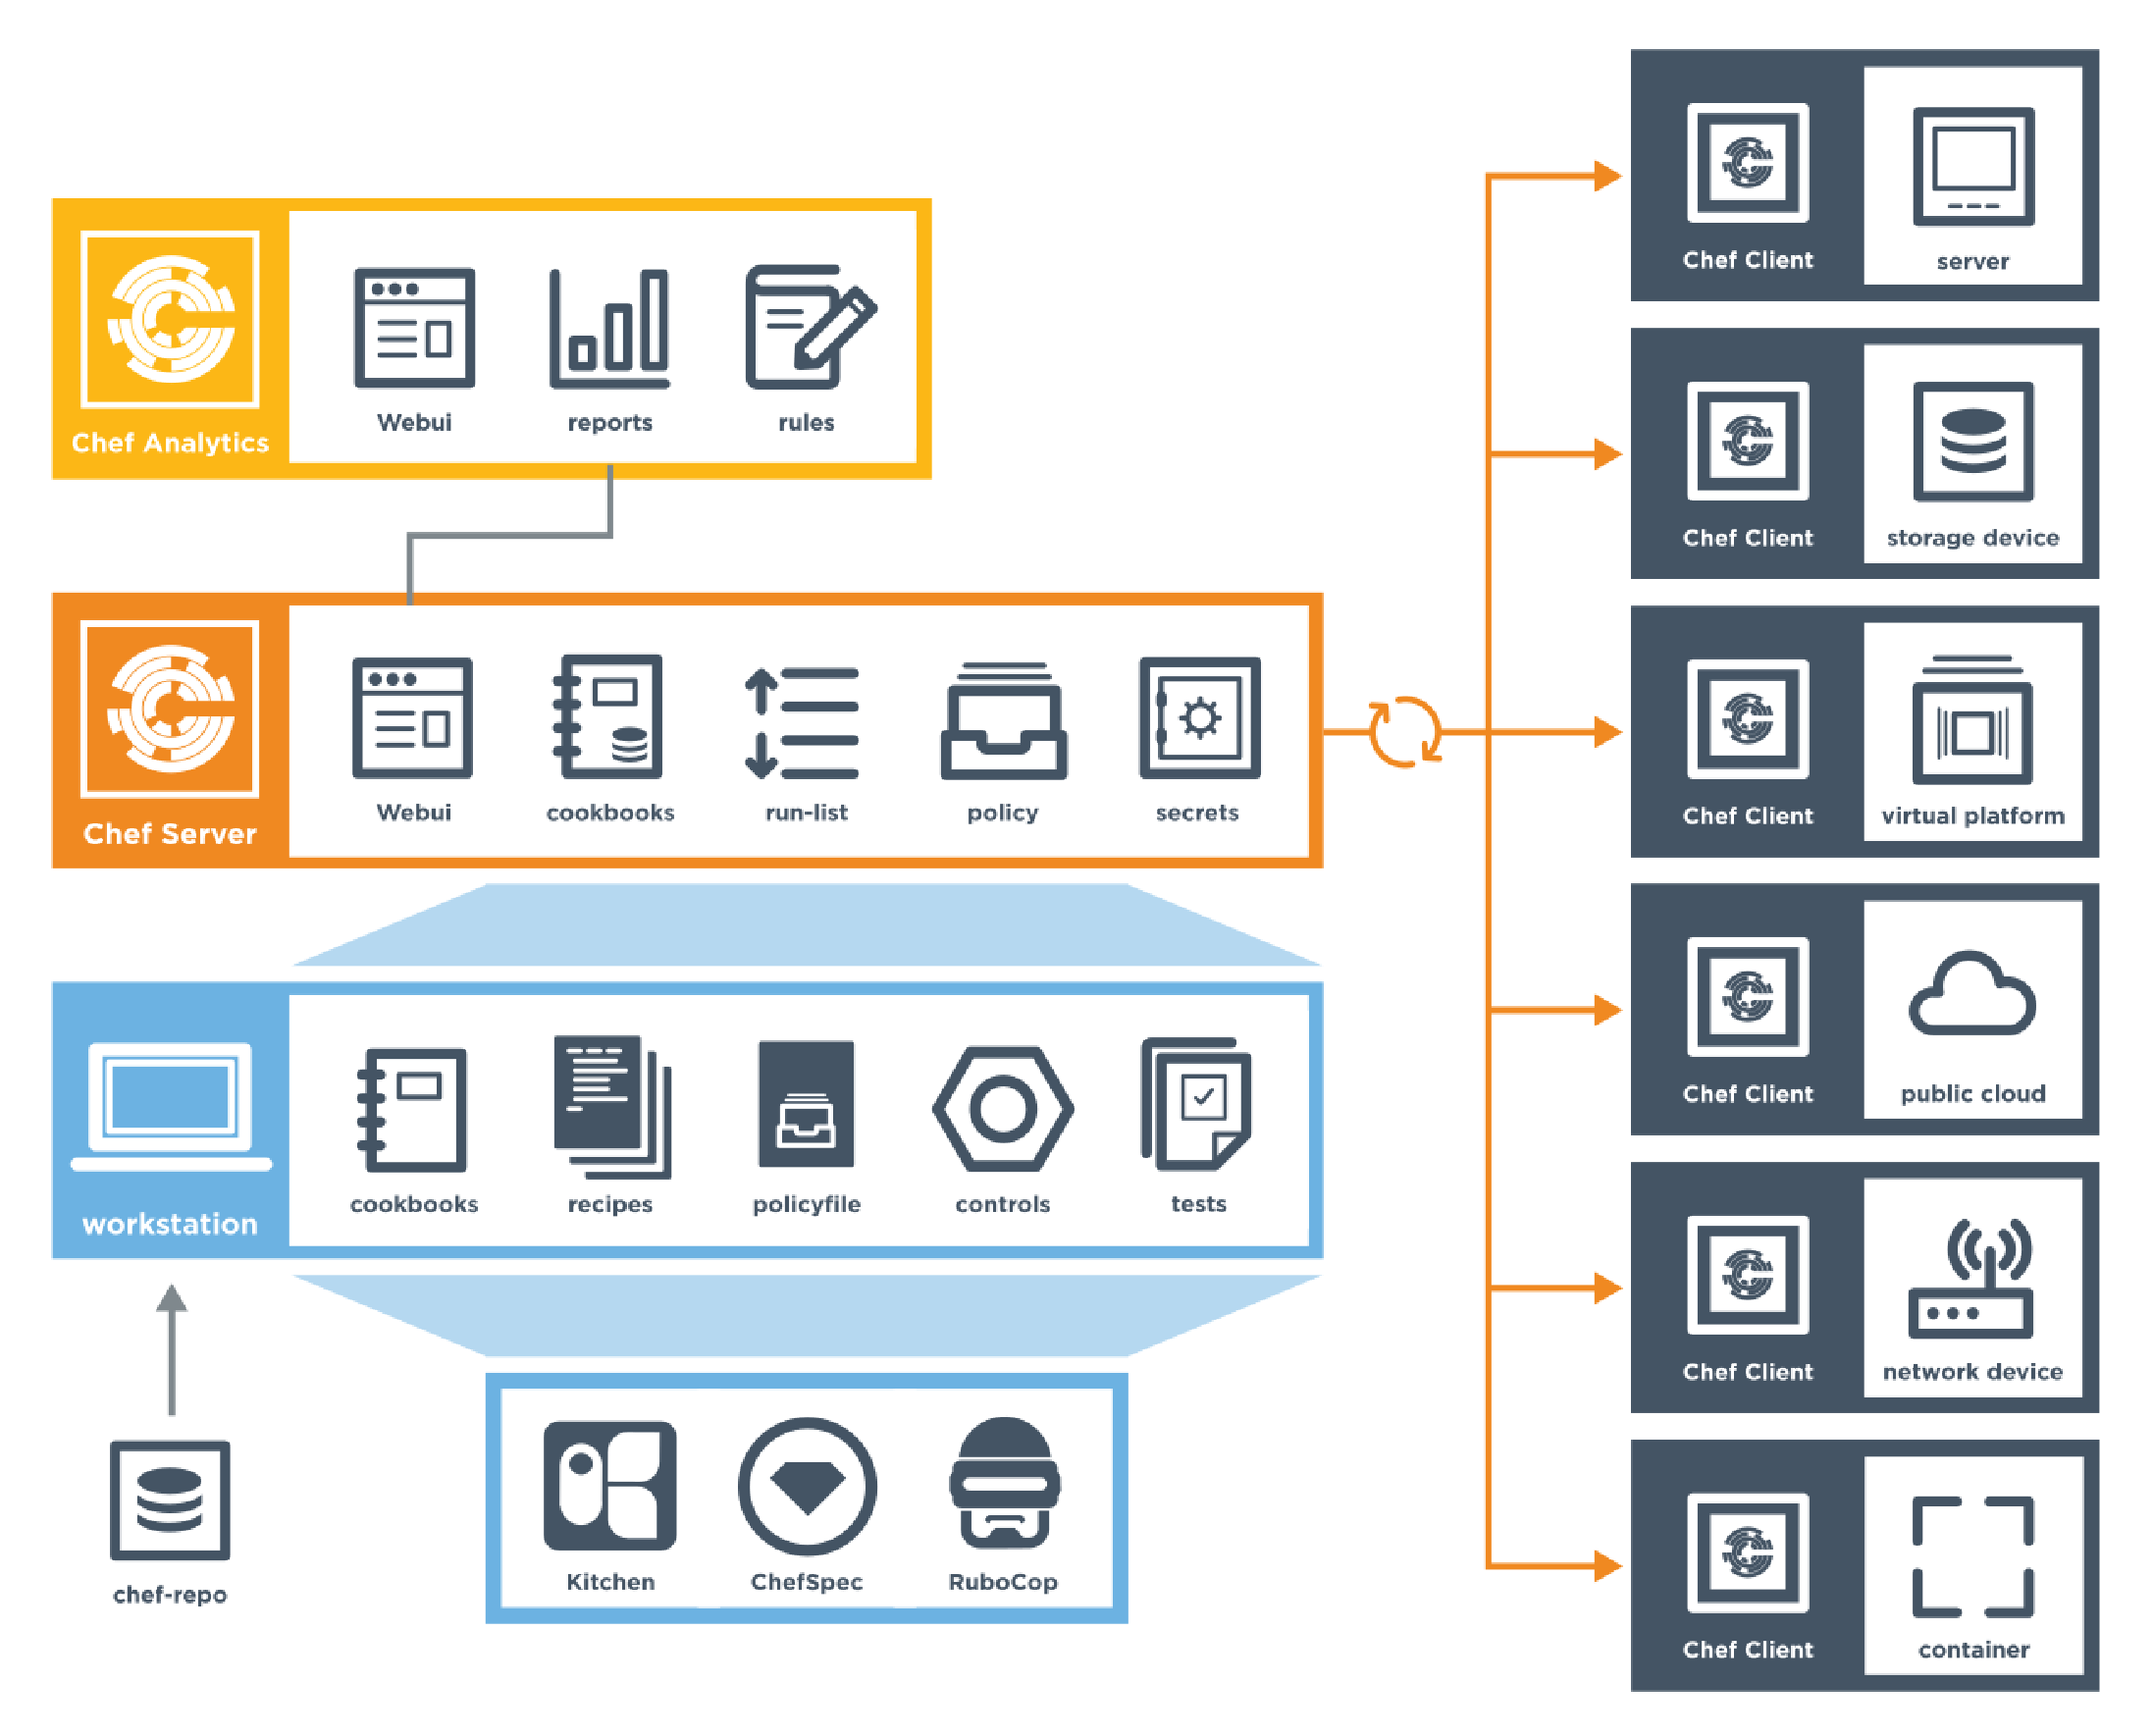
\includegraphics[width=\textwidth]{figuras/arch_chef.eps}
  \caption{Chef - Arquitetura de Componentes}
\end{figure}


